\chapter{Diseño}
\label{ch:diseno}

\section{Modelo UML de la sintaxis abstracta}
\lstsetocl

En la figura \ref{fig:modelo-ast} se muestra el diagrama de clases de
nuestra herramienta.

\begin{figure}
  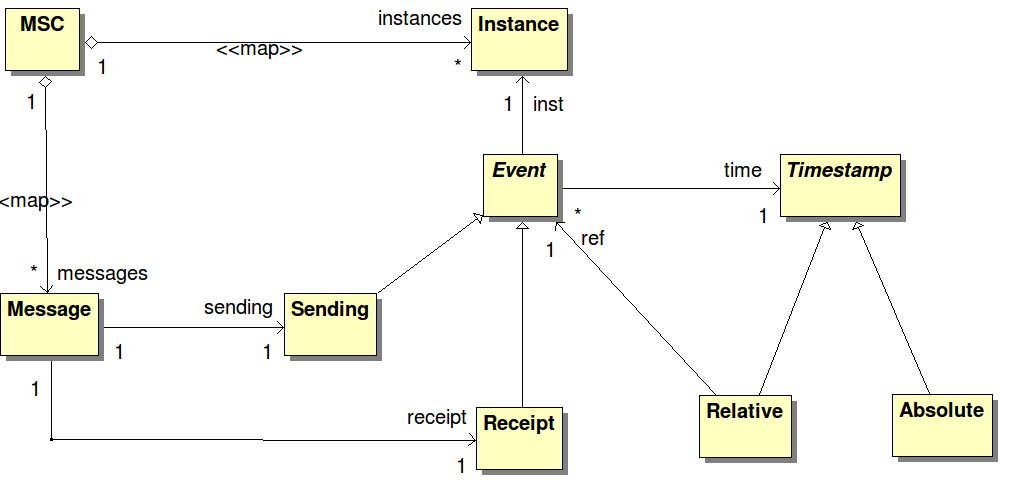
\includegraphics[width=1.0\linewidth]{./images/modelo-ast}
  \caption{Diagrama de clases}
  \label{fig:modelo-ast}
\end{figure}

\todo{AB:donde colocamos el diagrama de clases detallado?}

Visto el diagrama de clases, procedemos a explicar la representación
abstracta respecto a la concreta:
\begin{itemize}
\item La clase \textit{MSC} representa a nuestro MSC propiamente
  dicho. En él, almacenamos las instancias y mensajes que el usuario va
  introduciendo en la comunicación.
\item La clase \textit{Instance} representa las instancias
  \ref{sec:Instancias}  las cuales realizan la comunicación.
\item La clase \textit{Message} representa los mensajes
  \ref{sec:Mensajes} que forman la comunicación.
\item La clase \textit{Event} representa un evento de envío
  (\textit{Sending}) o recepción (\textit{Receipt}) dentro de la
  comunicación.
\item La clase \textit{Timestamp} representa los tiempos en que se
  efectúan los eventos. Como vimos \ref{sec:Tiempos} estos pueden ser
  absolutos (\textit{Absolute}) o relativos (\textit{Relative}).
\end{itemize}

\section{Arquitectura}

El diagrama de arquitectura, que podemos ver en la
figura~\ref{fig:diagrarquitectura}, representa a grandes rasgos el
funcionamiento de \textit{Progtalk}. Los procesos están representados
por círculos, y los datos por cuadrados.

\begin{figure}
  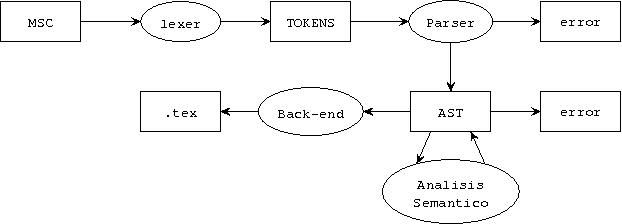
\includegraphics[scale=0.7]{./images/diag_arquitectura.png}
  \caption{Diagrama de arquitectura}
  \label{fig:diagrarquitectura}
\end{figure}

Básicamente la arquitectura de \textit{Progtalk} es la siguiente:
\begin{itemize}
\item En un primer lugar tenemos el analizador léxico. Su labor es ir
  tomando información del fichero de entrada carácter a carácter e ir
  agrupando en \textit{tokens} (unidad mínima de información que
  maneja posteriormente el analizador sintáctico).
\item Los tokens son enviados al analizador sintáctico, el cuál se
  encarga de parsear el fichero de entrada (es decir, va uniendo los
  tokens que va recibiendo y verifica que el fichero entrante esta
  escrito conforme al lenguaje diseñado para describir el universo del
  problema).  Durante el análisis sintáctico del fichero de entrada se
  hace necesario la creación de una serie de objetos los cuales sirven
  como almacenamiento intermedio de la información. La razón para
  hacer esto es la siguiente: imaginemos que estamos parseando una
  línea del fichero de entrada. Lo que el analizador sintáctico (a
  partir de ahora \textit{parser}) va a hacer es ir comparando la
  entrada con cada una de las reglas de dicho parser. Se irá creando
  un árbol sintáctico conforme avanza el parseo, y almacenando la
  información leída para que una vez se acepte la línea de entrada
  tengamos toda la información sobre dicha línea recopilada, y podamos
  almacenarla en el objeto\textit{msc} en el cual se almacena toda la
  comunicación antes de generar el fichero \textit{.tex}. El diagrama
  de clases correspondiente aparece representado en la
  figura~\ref{fig:diagparseo.png}.

\begin{figure}
  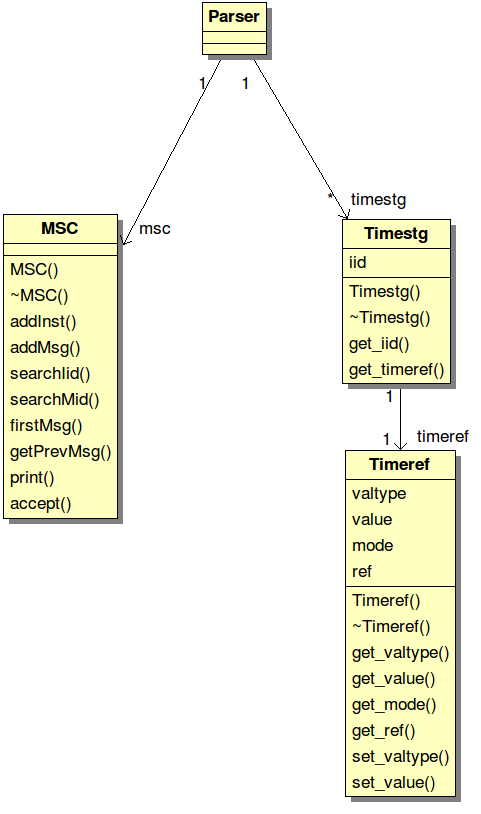
\includegraphics[scale=0.7]{./images/diagparseo.png}
  \caption{Diagrama de clases del proceso de almacenamiento durante el
  proceso de parsing.}
  \label{fig:diagparseo}
\end{figure}

\item Para verificar la consistencia de la comunicación tenemos el
  analizador semántico. En este punto, debemos explicar que parte de
  este análisis se ha realizado durante el análisis sintáctico, y
  parte se ha realizado tras la finalización de éste. La razón por la
  que tomamos esta decisión es que algunas verificaciones de
  consistencia, como por ejemplo la no duplicidad de identificadores,
  era fácil de empotrar dentro del código del analizador sintáctico,
  optimizando el funcionamiento de \textit{Progtalk} sin aumentar la
  complejidad del código, mientras que otras verificaciones como por
  ejemplo la consistencia de los tiempos de envío y recepción, eran
  suficientemente complejas como para diferir su procesado,
  simplificando así mucho el código.
\item Por ultimo tenemos el generador de código, que lee toda la
  comunicación procesada y almacenada en memoria, y la exporta al
  formato requerido por el usuario.
\end{itemize}

\section{Análisis Léxico}
Para implementar el analizador léxico (al cual hemos llamado
\textit{Scanner}) hemos usado flex++. Los tokens que hemos definido
para el universo de nuestro problema son:

\lstset{language=C,style=code}

\begin{itemize}
\item \lstinline{NUM: [0-9]} (cualquier número entero)
\item \lstinline{ID: [a-zA-Z][a-zA-Z0-9_]*} (cualquier identificador
  comenzado  en letra y formado por letras, números o el símbolo ''\_'')
\item\lstinline{ WHITE: [ \t]+} (cualquier espacio en blanco o tabulador)
\item \lstinline{STRING: \"[^\"\n]*\"} (cualquier conjunto de caracteres entre
  comillado salvo comillas o salto de línea)
\item \lstinline{EOLN: [\n]+} (uno o más saltos de línea)
\item \lstinline{INSTANCE: "instance"} (el literal \lstinline{instance})
\item \lstinline{OF: "of"} (el literal \lstinline{of})
\item \lstinline{MESSAGE: "message"} (el literal \lstinline{message})
\item \lstinline{FROM: "from"} (el literal \lstinline{from})
\item \lstinline{TO: "to"} (el literal \lstinline{to})
\item \lstinline{AT: "at"} (el literal \lstinline{@})
\item \lstinline{PLUS: "+"} (el literal \lstinline{+})
\item \lstinline{MINUS: "-"} (el literal \lstinline{-})
\item \lstinline{EXCLAMATION: "!"} (el literal \lstinline{!})
\item \lstinline{INTERROGATION: "?"} (el literal \lstinline{?})
\item \lstinline{SEMICOLON: ";"} (el literal \lstinline{;})
\item \lstinline!LEFT_BRACE: "{"! (el literal \lstinline!{!)
\item \lstinline!RIGHT_BRACE: "}"! (el literal \lstinline!}!)
\end{itemize}

\section{Análisis Sintáctico}

Para implementar el analizador sintáctico (al cual hemos llamado
\textit{Parser}) hemos usado \textit{bisonc++}. El proceso de parseo
es el siguiente. El objeto \textit{Parser} va tomando los tokens
enviados por \textit{Scanner} y comprueba que el lenguaje que esta
leyendo es un lenguaje correcto. En caso de no serlo se aborta el
proceso de parseo y el programa termina.

Las acciones semánticas en \emph{bisonc++} simplemente construyen los
nodos del árbol de sintaxis abstracta. Veamos un ejemplo de una de
nuestras acciones semánticas: \lstsetc
\todo{AB: Este codigo hay que revisarlo. Al hacer el pdf se sale de
  los margenes y queda francamente mal.}
\begin{lstlisting}
message:
     MESSAGE mid_opt string_opt origin_opt destiny_opt SEMICOLON EOLN
        { 
	  string * mid = $2;
          string * desc = $3;
          Timestg * orig = $4;
          Timestg * dest = $5;
        }
	  if (mid == NULL)
	    mid = new string("No_Info_Available");

	  if (desc == NULL)
	    desc = new string("");

	  if (orig == NULL)
	    {
	      std::cout << "ERROR: User didn't provide message's origin" 
			<< std::endl;
	      exit(-1);
	    }

	  if (dest == NULL)
	    {
	      std::cout << "ERROR: User didn't provide message's destiny" 

			<< std::endl;
	      exit(-1);
	    }
	     addMsg(*mid, *desc, orig->get_iid(), dest->get_iid(), 
		 orig->get_timeref(), dest->get_timeref());
	}
;
\end{lstlisting}

Se puede observar cómo el símbolo no terminal \lstinline{message} está
formado por el símbolo terminal \lstinline{MESSAGE} y a su vez por una
serie de símbolos no terminales que representan toda la información
que forma parte de un mensaje.

\section{Análisis Semántico}

En nuestro programa parte del análisis semántico se realiza de forma
paralela al análisis sintáctico y parte se realiza tras finalizar
éste. En concreto, las inconsistencias que se reconocen durante el
análisis sintáctico son:
\begin{itemize}
\item La declaración de varias instancias con igual identificador,
\item la declaración de varios mensajes con igual identificador,
\item la ausencia de elementos imprescindibles de un mensaje, como su
  origen o destino, \todo{AB: esto no sería más bien un error
    sintáctico mas que semántico?}
\item la referencia a una instancia que no ha sido declarada
  anteriormente.
\end{itemize}

El hecho de detectar estas inconsistencias nada más producirse, nos da
la ventaja de evitar el procesado de una comunicación errónea,
ahorrando tiempo y recursos.

Una vez terminado este proceso con éxito, pasamos a la segunda parte
del análisis semántico donde comprobaremos la consistencia en los
tiempos de envío y recepción de los mensajes así como la consistencia
en las referencias entre mensajes.

Hay dos razones por las que nos hemos realizado esta comprobación en
paralelo con el análisis sintáctico:
\begin{itemize}
\item Por un lado, durante la fase de análisis del problema, tomamos
  la decisión de intentar almacenar la información del fichero de
  entrada tan fielmente como fuera posible para así poder dar marcha
  atrás si lo deseáramos y obtener de nuevo el fichero de entrada a
  partir del la información parseada y almacenada. Esto implica que
  los tiempos relativos se almacenan como referencias y no como
  valores absolutos, lo que hace imposible comprobar su integridad
  hasta el final del parseo,
\item y por otro lado, comprendimos que el código del analizador
  sintáctico se volvería demasiado complejo y poco legible si
  finalmente incluíamos este tipo de verificaciones durante esta fase.
\end{itemize}

Para la implementación de esta parte del analizador semántico hemos
usado un patrón \textit{Visitor}~\cite{gof}, el cual nos permite
definir una nueva operación sin cambiar las clases de los elementos
sobre los que nuestra nueva operación actúa.

En la figura~\ref{fig:diagvisitor} se muestra el diagrama de clases que
representa a nuestro patrón \textit{Visitor}.

\begin{figure}
  \centering 
  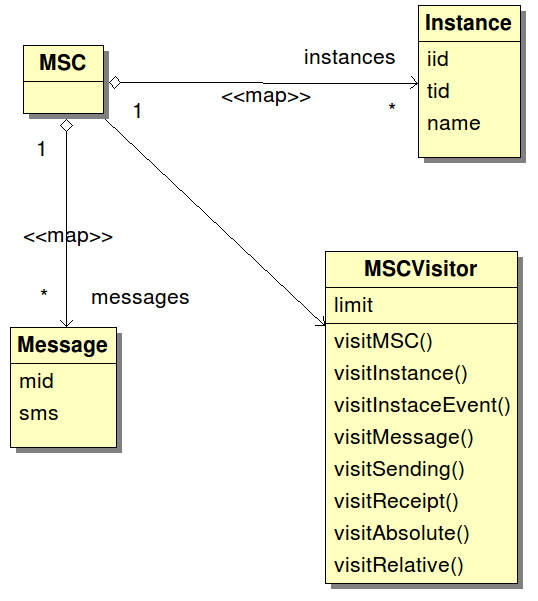
\includegraphics[scale=0.7]{./images/diag_visitor.png}
  \caption{Diagrama de clases de Visitor}
  \label{fig:diagvisitor}
\end{figure}

\todo{AB: explicaremos nuestro patron Visitor cuando lo corrijamos.}

\section{Generación de Código}

Para esta tarea hemos utilizado un patrón de diseño \textit{Visitor},
el cual recorre toda la información almacenada y a partir de ésta crea
un fichero \textit{.tex} que comp ilado en \textit{latex} nos dará una
representación gráfica de la comunicación.

\todo{AB:que tal si añadimos otro capitulo/sección donde metemos el
  ejemplo de lars con todos los diagramas?}

%%% Local Variables: 
%%% mode: latex
%%% TeX-master: "progtalk"
%%% TeX-PDF-mode: t
%%% ispell-local-dictionary: "castellano"
%%% End: 
